\section{Konzept zur Feature-Extraktion} \label{sec:Meth FeatExtr}
Für die Feature-Extraktion stehen Detektionsdatensätze und die Videos zur Verfügung. Mittels  Assoziationsmodul lassen sich Trajektorien generieren, aus denen sich ebenfalls Features extrahieren lassen. Grundlage für die Feature-Extraktion ist der Ereignisdatensatz, auf den sich die Tabelle \ref{tab:DatasetFeatExtr} bezieht. Ziel des Konzepts zur Feature-Extraktion ist es, einen Trainingsdatensatz zu generieren. Ebenfalls ist das Konzept so zu entwerfen, dass es sich modular in die Vorverarbeitung des Gesamtkonzepts integrieren lässt (\autoref{sec:Meth gesamtkonzept}). Das Konzept zur Generierung des Trainingsdatensatzes ist als Blockdiagramm in der Abbildung \ref{fig:KonzeptFeatExtr} zu sehen. Anschließend werden die einzelnen Module im Detail beschrieben.

\begin{figure}[htb]
    \centering
    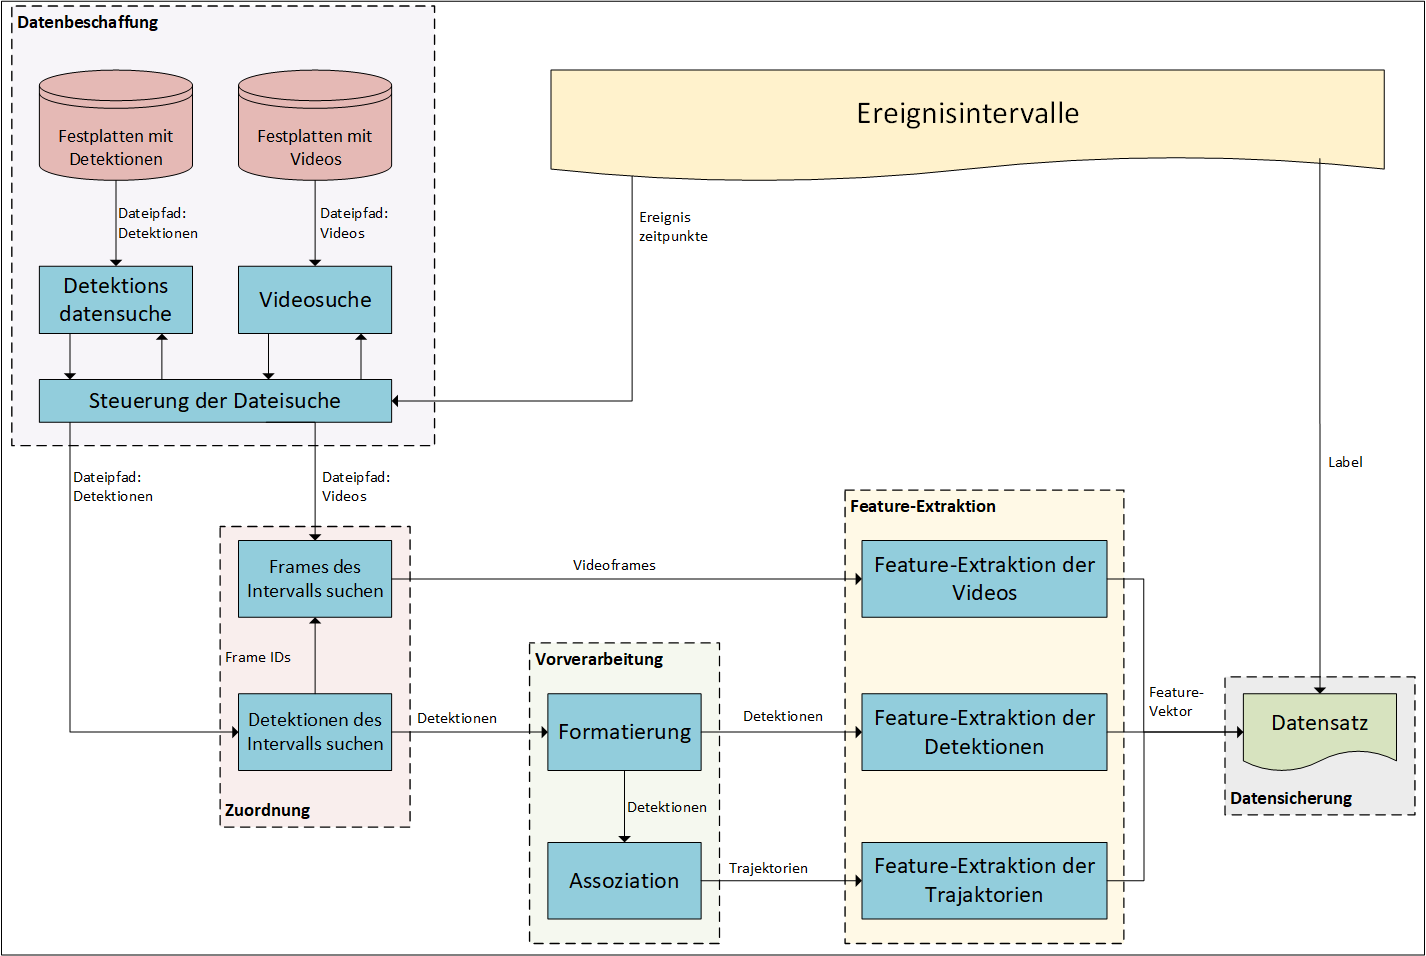
\includegraphics[width=\textwidth]{img/Grafiken/Konzept Feature-Extraktion.png}
    \caption[Blockdiagramm des Konzepts zur Feature-Extraktion.]{Blockdiagramm des Konzepts zur Feature-Extraktion. Das Konzept lässt sich in fünf Module unterteilen: die Datenbeschaffung, die Datenzuordnung, eine Vorverarbeitung, die Feature-Extraktion und die Datensicherung. Als Eingabe erhalten die Module den Ereignisdatensatz.}
    \label{fig:KonzeptFeatExtr}
\end{figure}

\begin{quote}
\par
\textbf{Datenbeschaffung}\par
Die Aufgabe der Datenbeschaffung ist es, die passenden Dateien zu einem Ereignis herauszusuchen. Es ist das gleiche Hilfsmodul wie in der Ereignisverifizierung (\autoref{sec:Meth Labeling}). Als Eingabe erhält es den Startzeitpunkt eines Ereignisses. Als Ausgabe gibt es den Dateipfad zu der Videodatei und dem Detektionsdatensatz zurück, die zu dem Zeitpunkt passen. \dubpar

\textbf{Zuordnung der Daten zu dem Ereignis}\par
Aus der Detektionsdatei werden basierend auf den Zeitstempeln die Einträge herausgesucht, welche zu dem Zeitraum des Ereignisses passen. In diesen Einträgen findet sich die ID der Frames zum dazugehörigen Video. Darüber lassen sich die passenden Frames identifizieren. Als Eingabe benötigt das Modul den Dateipfad zu einer Videodatei, den Dateipfad zu einem Detektionsdatensatz, einen Startzeitpunkt und einen Endzeitpunkt eines Ereignisses. Die Ausgabe der Zuordnung sind die zum Ereignis passenden Detektionseinträge und Frames. \dubpar

\textbf{Vorverarbeitung}\par
Die Vorverarbeitung ist für die Extraktion der Features aus den Detektionen und den Trajektorien notwendig. Zunächst sind die Detektionen zu formatieren. Im Detektionsdatensatz sind die Detektionen frameweise abgespeichert. Damit ist gemeint, dass jeder Eintrag im Detektionsdatensatz sich auf ein Frame im Video bezieht. Für die Weiterverarbeitung ist jedoch eine detektionsweise Formatierung praktischer. Damit ist gemeint: jede Detektion erhält einen eigenen Eintrag. Diese formatierten Detektionen werden dem Assoziationsmodul übergeben, das wiederum die Trajektorien zum Ereignis generiert. Als Eingabe erhält die Vorverarbeitung die Detektionen aus einer Detektionsdatei. Die Ausgabe sind die Trajektorien und die formatierten Detektionen. \dubpar

\textbf{Feature-Extraktion}\par
In der Feature-Extraktion werden die Features berechnet. Sie ist aufgebaut aus drei Programmen, die sich jeweils um eine andere Datenquelle kümmern. Ein Programm erhält die Frames des Videos und extrahiert Features aus dem Bildmaterial. Ein weiteres Programm erhält die formatierten Detektionsdaten und extrahiert daraus Features. Das letzte Programm ist für die Trajektorien zuständig. Dieses bekommt die Trajektorien übergeben und berechnet daraus Features. Jedes der Programme gibt die jeweiligen Features aus. Diese laufen im Featurevektor zusammen. \dubpar

\textbf{Datensicherung}\par
In der Datensicherung wird der Featurevektor aus der Feature-Extraktion entgegengenommen und mit dem Label des Ereignisses versehen. Label und Features werden in einem Datensatz abgelegt. 

\end{quote}

Der Prozess ist automatisiert. Wird dem Konzept ein Ereignisdatensatz übergeben, wird automatisch durch die Ereignisse iteriert. Der Datensatz, in dem Labels und Features zusammenlaufen, kann für das Modelltraining verwendet werden oder für die Konstruktion weiterer Features. In Bezug auf das Gesamtkonzept des Moduls zur Verhaltensklassifikation ist zu sehen, dass die Module der Feature-Extraktion und der Vorverarbeitung die gleichen Datenströme erhalten wie die Vorverarbeitung im Gesamtkonzept. Somit sind diese Module direkt in das Gesamtkonzept integrierbar.